\chapter{The Electron}

\chapterprecis{R.\ A.\ Millikan}

\makeoddhead{myheadings}{\emph{Millikan}}{}{\thepage}
\makeevenhead{myheadings}{\thepage}{}{\emph{The Electron}}

\section*{Remarks}

\indent
We turn now to the examination of ``charge'' itself, in particular to
the question whether charge is discrete or continuous in its ultimate
composition. That question was ef\-fec\-tive\-ly answered with R.\ A.\ 
Millikan's discovery of a fundamental unit of charge---the so-called
``electron.''

The instrument Millikan employed for that delicate task of measurement
is a tiny droplet of oil bearing a minute electrical charge, alternately
hoisted up by an applied electric field, then allowed to fall back down
under its own weight with the field turned off. From observations of the
motion of such drops Millikan was able, first, to show that a
fundamental unit of charge \emph{exists}; second, to determine the
magnitude of that unit.

In the selection that follows, Millikan takes as granted the equations
governing the motion of the oil drop. Therefore the first phase in our
reasoning must be to work out in a general way the forces that act on
the drop and to derive the equation of its motion under those forces. It
will be assumed at this point that the size and mass of the drop are
known; actually their determination constitutes an important second
phase of the analysis.

\begin{figure}[h]
  \begin{center}
    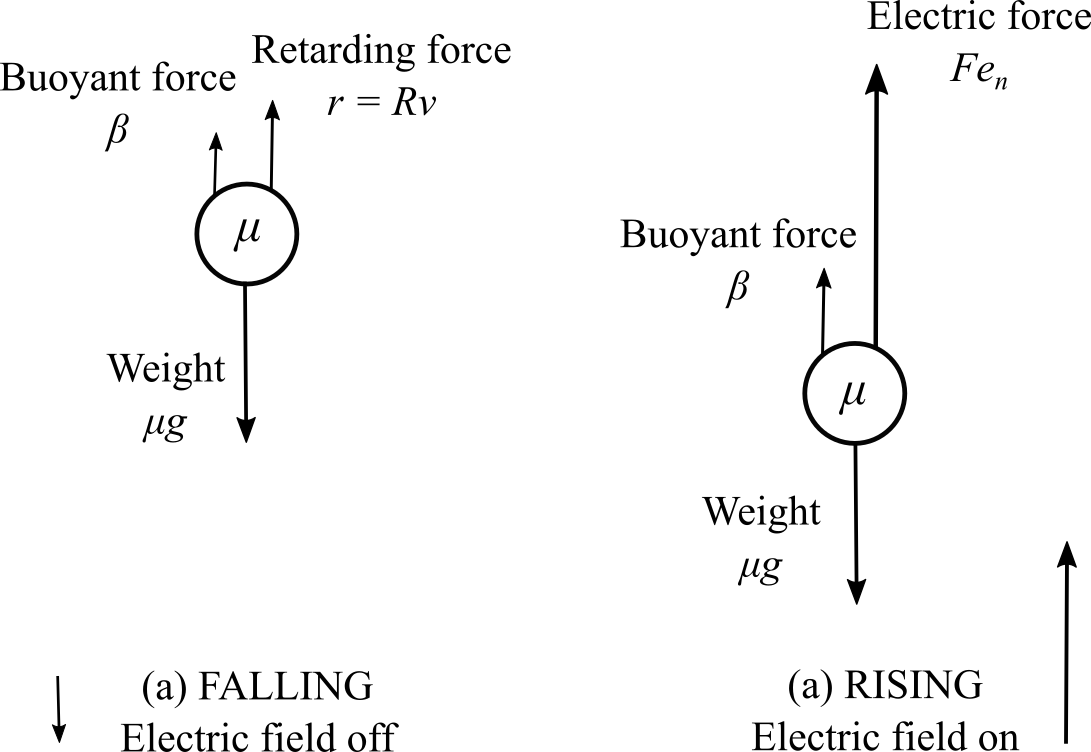
\includegraphics[width=3.63667in]{images/03_millikan/drops.png}
  \end{center}
\end{figure}

The forces which act on a falling drop in the absence of an electric
field are sketched on the left side of the diagram, marked (a). The mass 
of the drop is $\mu$ and the weight is therefore $\mu g$. The drop falls 
through the air, which we shall regard as a very thin homogeneous fluid that 
both buoys up a body and resists motion through itself. We also assume, with 
Millikan, that this resisting force is \emph{directly proportional to the 
velocity} of the moving drop. This proportionality characterizes the special 
type of friction called a ``viscous'' force, exerted by a ``viscous'' fluid 
on any body moving through it. The measure of a fluid's capacity for
applying such a force is called its ``viscosity.'' Millikan had good
reason to believe that air exhibited this viscosity quite strictly.

With some constant of proportionality, $R$, then, the viscous force
$r$ resisting the droplet's fall will be

\begin{equation*}\tag{3.1}
r = Rv
\end{equation*}
%
as shown in Fig. (a).

At the same time, the drop is buoyed up by a force equal to the weight
of air which it displaces.\footnote{Archimedes, \emph{On Floating
  Bodies}, I, Prop.\ 7.} Thus a droplet of volume $V$ will have mass
$\mu = V\sigma$, but it will displace a mass $V\rho$ of air,
where $\sigma$ is the density of the oil and $\rho$ is the density of
the air. Hence the three forces acting on the falling drop are:

\begin{align*}
\text{Weight}\quad W & = V\sigma g\\
\text{Buoyancy}\quad \beta & = V\rho g\\
\text{Retarding force}\quad r &= Rv\\
\end{align*}
%
for a total downward force $f$ of
%
\begin{align*}
f &= V\sigma g-V\rho g-Rv\\
 &= V(\sigma-\rho)g-Rv\\
\end{align*}

On analogy with $V\sigma$, the actual mass of the oil drop, Millikan
will call $V(\sigma-\rho)$ in the expression above the
``effective'' grav\-i\-ta\-tion\-al mass, $m$---as though the reduced
downward tendency of the drop in the buoyant medium were due to a
reduced grav\-i\-ta\-tion\-al mass $m = V(\sigma-\rho)$
rather than, as is actually the case, to the presence of an upward
buoyant force $\beta = V\rho g$. The expression for the net downward
force can then be written
\begin{equation*}\tag{3.2}
f = mg - Rv
\end{equation*}
where $m = V(\sigma-\rho)$. There will be a downward
acceleration---that is, a continuing increase in velocity $v$---so
long as the resistance $Rv$ of the medium is less than the
effective weight $mg$.

However, as the velocity of the drop increases, so will the resistance;
as $Rv$ increases it will approach $mg$ and the net force
$f$ will approach zero, as is clear from equation (3.2) above. The
acceleration will become very small, and the droplet will continuously 
approach the \emph{constant} velocity $v_1$,\footnote{In practice, the drop
almost immediatley accelerates to a velocity immeasurably close to its terminal 
velocity.} characterized as the velocity at which
\begin{equation*}
Rv = mg.
\end{equation*}
%
This gives
\begin{equation*}\tag{3.3}
v_1 = \frac{mg}{R}.
\end{equation*}

Suppose now that the droplet bears electric charge $e_n$. In the
absence of an electric field, that charge will not affect the drop's
motion. But when a field $F$ tending to raise the drop is applied,
an upward force $Fe_n$ will act on the drop; and if it is strong
enough to overbalance the effective weight of the drop, the drop will
stop falling and begin to rise. Then while the drop is rising both the
effective weight and the viscous force will be \emph{downwards}, and
there will act on the drop (see Fig. (b)) a net \emph{upward} force
equal to
\begin{equation*}
Fe_n - mg - Rv.
\end{equation*}
Then by an argument similar to that for the drop when falling, the
rising drop will shortly attain a constant upward velocity $v_2$,
where
\begin{equation*}\tag{3.4}
v_2=\frac{Fe_n - mg}{R}
\end{equation*}
It is a striking characteristic of motion in a viscous medium that a
body under the action of a constant force attains a \emph{constant
velocity proportional to that force}.

Equations (3.3) and (3.4) constitute all the theory that Millikan
requires to establish from his observations that the electron
\emph{exists}; although calculation of its \emph{quantity} involves, as
we shall see, considerably more reasoning. Actually Millikan uses the
\emph{quotient} of equation (3.3) by equation (3.4), which is
\begin{center}
\begin{align*}\tag{1}
\frac{v_1}{v_2} = \frac{mg}{Fe_n - mg} \quad\text{or}\quad & e_n = \frac{mg}{Fv_1}(v_1 + v_2)
\end{align*}
\end{center}
It will be called equation (9) in the selection that follows.

A final remark: unlike Thomson (who had to deal with both electric and
magnetic qualities in his calculations), Millikan, who deals with the
electron only in its e\-lec\-tro\-stat\-ic relations, accordingly uses the
\emph{e\-lec\-tro\-stat\-ic system of units} (e.s.u.) in what we are about to
read. Thus he will eventually state his fundamental unit of charge in
\emph{stat\-cou\-lombs.} In order to relate Millikan's and Thomson's
results, recall that the electromagnetic and the e\-lec\-tro\-stat\-ic systems
of units are related by the constant \emph{c} (the speed of light in 
centimeters per second), so that one abcoulomb
equals $3.00 \times 10^{10}$ stat\-cou\-lombs. (See Appendix below
for a fuller discussion of the relation between the ``e\-lec\-tro\-stat\-ic''
and ``electromagnetic'' system of units.)

\section*{The Electron\\ {\large R.\ A.\ Millikan}}

\subsection*{General Proof of the Atomic Nature of Electricity\footnote{[Chapter IV of \emph{The Electron}, University of
  Chicago Press (1924). Although we are reading his 1924 account,
  Millikan developed the methods here described from 1909 to 1913.]}}


Although the ``balanced droplet method'' just described\footnote{{[}Millikan
  here refers to an earlier technique, omitted here.{]}} had eliminated
the chief sour\-ces of uncertainty which inhered in preceding work on
\emph{e} and had made it possible to assert with much confidence that
the unit charge was a real physical entity and not merely a
``statistical mean,'' it was yet very far from an exact method of
studying the properties of gaseous ions. The sour\-ces of error or
uncertainty which still inhered in it arose from (1) the lack of
stagnancy in the air through which the drop moved; (2) the lack of
perfect uniformity of the electrical field used; (3) the gradual
evaporation of the drops, rendering it impossible to hold a given drop
under observation for more than a minute or to time a drop as it fell
under gravity alone through a period of more than five or six seconds;
and (4) the assumption of the validity of Stokes's Law.

The method which was devised to replace it was not only entirely free
from all of these limitations, but it constituted an entirely new way of
studying ionization and one which at once yielded important results in a
considerable number of directions. This chapter deals with some of these
by-products of the determination of \emph{e} which are of even more
fundamental interest and importance than the mere discovery of the exact
size of the electron.

\subsection*{I. Isolation of Individual Ions and Measurement of Their Relative Charges}

In order to compare the charges on different ions, the procedure adopted
was to blow with an ordinary commercial atomizer an oil spray into the
chamber C (Fig. 3). The air with which this spray was blown was first
rendered dust-free by passage through a tube containing glass wool. The
minute droplets of oil constituting the spray, most of them having a
radius of the order of a one-thousandth of a millimeter, slowly fell in
the chamber C, and occasionally one of them would find its way through
the minute pinhole \emph{p} in the middle of the circular brass plate M,
\begin{figure}[h]
  \begin{center}
    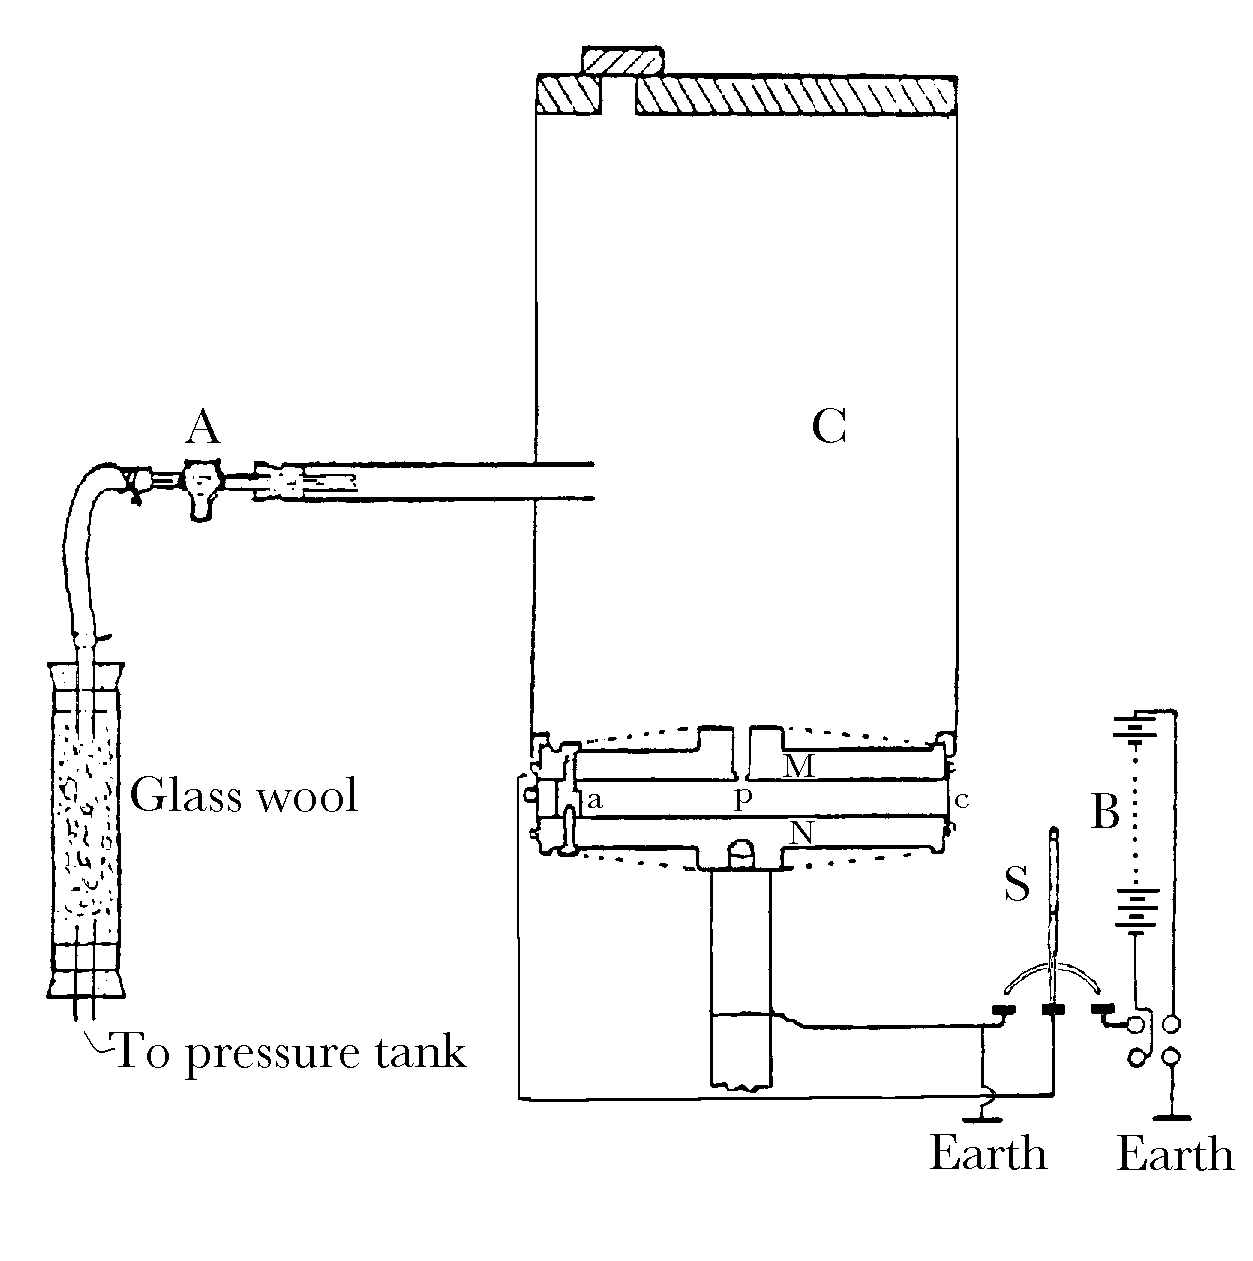
\includegraphics[width=0.6\textwidth]{images/03_millikan/image013.png}
  \end{center}
  \caption*{Figure 3}
\end{figure}
22 cm in diameter, which formed one of the plates of the air condenser.
The other plate, N, was held 16 mm. beneath it by three ebonite posts
\emph{a}. By means of the switch S these plates could be charged, the
one positively and the other negatively, by making them the terminals of
a 10,000-volt storage battery B, while throwing the switch the other way
(to the left) short-circuited them and reduced the field between them to
zero. The oil droplets which entered at \emph{p} were illuminated by a
powerful beam of light which passed through diametrically opposite
windows in the encircling ebonite strip \emph{c}. As viewed through a
third window in \emph{c} on the side toward the reader, it appeared as a
bright star on a black background. These droplets which entered \emph{p}
were found in general to have been strongly charged by the frictional
process involved in blowing the spray, so that when the field was thrown
on in the proper direction they would be pulled up toward M. Just before
the drop under observation could strike M the plates would be
short-circuited and the drop allowed to fall under gravity until it was
close to N, when the direction of motion would be again reversed by
throwing on the field. In this way the drop would be kept traveling back
and forth between the plates. The first time the experiment was tried an
ion\footnote{{[}``Ion'' was Faraday's term for the particles of matter
  which seemed, in electrolysis, to migrate from one region of the
  solution to another. Although Faraday himself distrusted the atomic
  view, researchers of a later generation collected much evidence that
  ``ions'' were actually \emph{electrically-charged atoms} (or groups of
  atoms), which were not only found in electrolytes but could also be
  produced in gases by various causes including x-rays and the presence
  of radioactive substances. In an earlier chapter of \emph{The
  Electron}, Millikan wrote: ``In a word, then, the act of ionization in
  gases appears to consist in the detachment from a neutral atom of one
  or more negatively charged particles, called by Thomson
  \emph{corpuscles}. The residuum of the atom is of course positively
  charged\ldots. The detached corpuscle must soon attach itself, in a
  gas at ordinary pressure, to a neutral atom.'' Thus some of the air
  molecules in Millikan's chamber carry either a positive or a negative
  charge, and it is these charged molecules---ions---that periodically
  collide with the oil drop and yield to it whatever charges they
  bear.{]}} was caught within
%
\begin{center}
\begin{tabular}{S c c c c S}
\multicolumn{6}{c}{\hspace{2em} TABLE IV}\\
$t_g$ & & & & $t_F$\\
13.6 & & & & 12.5\\
13.8 & & & & 12.4&\\
13.4 & & & & 21.8&\\
13.4 & & & & 34.8&\\
13.6 & & & & 84.5&\\
13.6 & & & & 85.5&\\
13.7 & & & & 34.6&\\
13.5 & & & & 34.8&\\
13.5 & & & & 16.0&\\
13.8 & & & & 34.8&\\
13.7 & & & & 34.6&\\
13.8 & & & & 21.9&\\
13.6&\\
13.5&\\
13.4&\\
13.8&\\
13.4&\\
\hline
\text{Mean} 13.595&\\
\end{tabular}
\end{center}
%
a few minutes, and the fact of its capture was signaled to the observer
by the change in the speed with which {[}the oil drop{]} moved up when
the field was on. The significance of the experiment can best be
appreciated by examination of the complete record of one of the early
experiments when the timing was done merely with a stop watch.

The column headed $t_g$ gives the successive times which the droplet
required to fall [under the force of gravity, $g$] between two fixed cross-hairs in the observing
telescope whose distance apart corresponded in this case to an actual
distance of fall of .5222 cm. It will be seen that these numbers are all
the same within the limits of error of a stop-watch measurement. The
column marked $t_F$ gives the successive times which the droplet
required to rise under the influence of the electrical field [$F$] produced by
applying in this case 5,051 volts of potential difference to the plates
M and N. It will be seen that after the second trip up, the time changed
from 12.4 to 21.8, indicating, since in this case the drop was positive,
that a negative ion had been caught from the air. The next time recorded
under $t_F$, namely, 34.8, indicates that another negative ion had
been caught. The next time, 84.5, indicates the capture of still another
negative ion. This charge was held for two trips, when the speed changed
back again to 34.6, showing that a positive ion had now been caught
which carried precisely the same charge as the negative ion which before
caused the inverse change in time, i.e., that from 34.8 to 84.5.

In order to obtain some of the most important consequences of this and
other similar experiments we need make no assumption further than this,
that the velocity with which the drop moves is proportional to the force
acting upon it and is independent of the electrical charge which it
carries. Fortunately this assumption can be put to very delicate
experimental test, as will presently be shown, but introducing it for
the time being as a mere assumption, as Townsend, Thomson, and Wilson
had done before, we get
%
\begin{center}
\begin{align*}\tag{9}
\frac{v_1}{v_2} = \frac{mg}{Fe_n-mg} \quad\text{or}\quad & e_n = \frac{mg}{Fv_1}(v_1+v_2)
\end{align*}
\end{center}
%
The negative sign is used in the denominator because $v_2$ will for
convenience be taken as positive when the drop is going up in the
direction of \emph{F}, while $v_1$ will be taken as positive when it
is going down in the direction of \emph{g}. $e_n$ denotes the charge
on the drop, and must not be confused with the charge on an ion. If now
by the capture of an ion the drop changes its charge from $e_n$ to
$e_{n'}$, then the value of the captured charge $e_i$ is
\begin{equation*}\tag{10}
e_i = e_{n'}-e_n=\frac{mg}{Fv_1}(v_{2}'-v_2)
\end{equation*}
and since $mg/Fv_1$ is a constant for this drop, any charge which it
may capture will always be proportional to ($v_{2}'-v_2$),
that is, to the change produced in the velocity in the field \emph{F} by
the captured ion. The successive values of $v_2$ and of ($v_{2}'-v_2$) 
are shown in Table V.

\begin{table}[htp]
\centering
\begin{minipage}{\textwidth}
\centering
\begin{tabular}{ c c }
  \multicolumn{2}{c}{TABLE V\footnote{[The bracketed numbers are our corrections of typos
  in Millikan's original table.]}}\\
  $v_2$ & $ (v'_2 - v_2)$\\
  &\\
  $\frac{.5222}{12.45} = .04196$ & \multirow{3}{*}{$\biggr\} .01806 \div 2 = .00903$}\\
  &\\
  $\frac{.5222}{{[}21.85{]}} = .02390$ & \multirow{3}{*}{$\biggr\} .00885 \div 1 = .00885$}\\
  &\\
  $\frac{.5222}{34.7} = .01505$ &\multirow{3}{*}{$\biggr\} .00891 \div 1 = .00891$}\\
  &\\
  $\frac{.5222}{85.0} = .006144$ &\multirow{3}{*}{$\biggr\} .00891 \div 1 = .00891$}\\
  &\\
  $\frac{.5222}{34.7} = .01505$ &\multirow{3}{*}{$\biggr\} .01759 \div 2 = .00880$}\\
  &\\
  $\frac{.5222}{16.0} = .02364$ &\multirow{3}{*}{$\biggr\} .01759 \div 2 = .00880$}\\
  &\\
  $\frac{.5222}{34.7} = .01505$ &\multirow{3}{*}{$\biggr\} [.00885 \div 1 = .00885]$}\\
  &\\
  $\frac{.5222}{21.85} = .02390$ &\\
\end{tabular}
\end{minipage}
\end{table}

It will be seen from the last column that within the limits of error of
a stop-watch measurement, all the charges captured have exactly the same
value save in three cases. In all of these three the captured charges
were just twice as large as those appearing in the other changes.
Relationships of exactly this sort have been found to hold absolutely
without exception, no matter in what gas the drops have been suspended
or what sort of droplets were used upon which to catch the ions. In many
cases a given drop has been held under observation for five or six hours
at a time and has been seen to catch not eight or ten ions, as in the
above experiment, but hundreds of them. Indeed, I have observed, all
told, the capture of many thousands of ions in this way, and in no case
have I ever found one the charge of which, when tested as above, did not
have either exactly the value of the smallest charge ever captured or
else a very small multiple of that value. \emph{Here, then, is direct,
unimpeachable proof that the electron is not a ``statistical mean,'' but
that rather the electrical charges found on ions all have either exactly
the same value or else small exact multiples of that value.}

\subsection*{II. Proof That All Static Charges Both on Conductors and Insulators Are
Built Up of Electrons}

The foregoing experiment leads, however, to results of much more
fundamental im\-por\-tance than that mentioned in the preceding section. The
charge which the droplet had when it first came under observation had
been acquired, not by the capture of ions from the air, but by the
ordinary frictional process involved in blowing the spray. If then
ordinary static charges are built up of electrons, this charge should be
found to be an exact multiple of the ionic charge which had been found
from the most reliable measurement shown in Table V to be proportional
to the velocity .00891. This initial charge $e_n$ on the drop is
seen from equations (9) and (10) to bear the same relation to ($v_1$
+ $v_2$) which the ionic charge $e_{n'} - e_n$ bears to
($v_{2}' - v_2$). Now, $v_1 = .5222\div13.595 = .03842$, hence
$v_1 + v_2 = .03842 + .04196 = .08038$. Dividing this by 9 we
obtain .008931, which is within about one-fifth of 1 per cent of the
value found in the last column of Table V as the smallest charge carried
by an ion. \emph{Our experiment has then given us for the first time a
means of comparing a frictional charge with the ionic charge, and the
frictional charge has in this instance been found to contain exactly 9
electrons.} A more exact means of making this comparison will be given
presently, but suffice it to say here that experiments like the
foregoing have now been tried on thousands of drops in different media,
some of the drops being made of non-conductors like oil, some of
semi-conductors like glycerin, some of excellent metallic conductors
like mercury. In every case, without a single exception, the initial
charge placed upon the drop by the frictional process, and all of the
dozen or more charges which have resulted from the capture by the drop
of a larger or smaller number of ions, have been found to be exact
multiples of the smallest charge caught from the air. Some of these
drops have started with no charge at all, and one, two, three, four,
five, and six elementary charges or electrons have been picked up.
Others have started with seven or eight units, others with twenty,
others with fifty, others with a hundred, others with a hundred and
fifty elementary units, and have picked up in each case a dozen or two
of elementary charges on either side of the starting point, so that in
all, drops containing every possible number of electrons between one and
one hundred and fifty have been observed and the number of electrons
which each drop carried has been accurately counted by the method
described. When the number is less than fifty there is not a whit more
uncertainty about this count than there is in counting one's own fingers
and toes. It is not found possible to determine with certainty the
number of electrons in a charge containing more than one hundred or two
hundred of them, for the simple reason that the method of measurement
used fails to detect the difference between 200 and 201, that is, we
cannot measure $v_{2}' - v_2$ with an accuracy greater than
one-half of 1 per cent. But it is quite inconceivable that large charges
such as are dealt with in commercial applications of electricity can be
built up in an es\-sen\-tially different way from that in which the small
charges whose electrons we can count are found to be. Furthermore, since
it has definitely been proved that an electrical current is nothing but
the motion of an electrical charge over or through a conductor, it is
evident that the experiments under consideration furnish not only the
most direct and convincing of evidence that all electrical charges are
built up out of these very units which we have been dealing with as
individuals in these experiments, but that all electrical currents
consist merely in the transport of these electrons through the
conducting bodies.

In order to show the beauty and precision with which these multiple
relationships stand out in all experiments of this kind, a table
corresponding to much more precise measurements than those given
heretofore is here introduced (Table VI). The times of fall and rise
shown in the first and second columns were taken with a Hipp chronoscope
reading to one-thousandths of a second. The third column gives the
reciprocals of these times. These are used in place of the velocities
$v_2$ in the field, since distance of fall and rise is always the
same. The fourth column gives the successive changes in speed due to the
capture of ions. These also are expressed merely as time reciprocals.

\begin{figure}[h]
  \begin{center}
    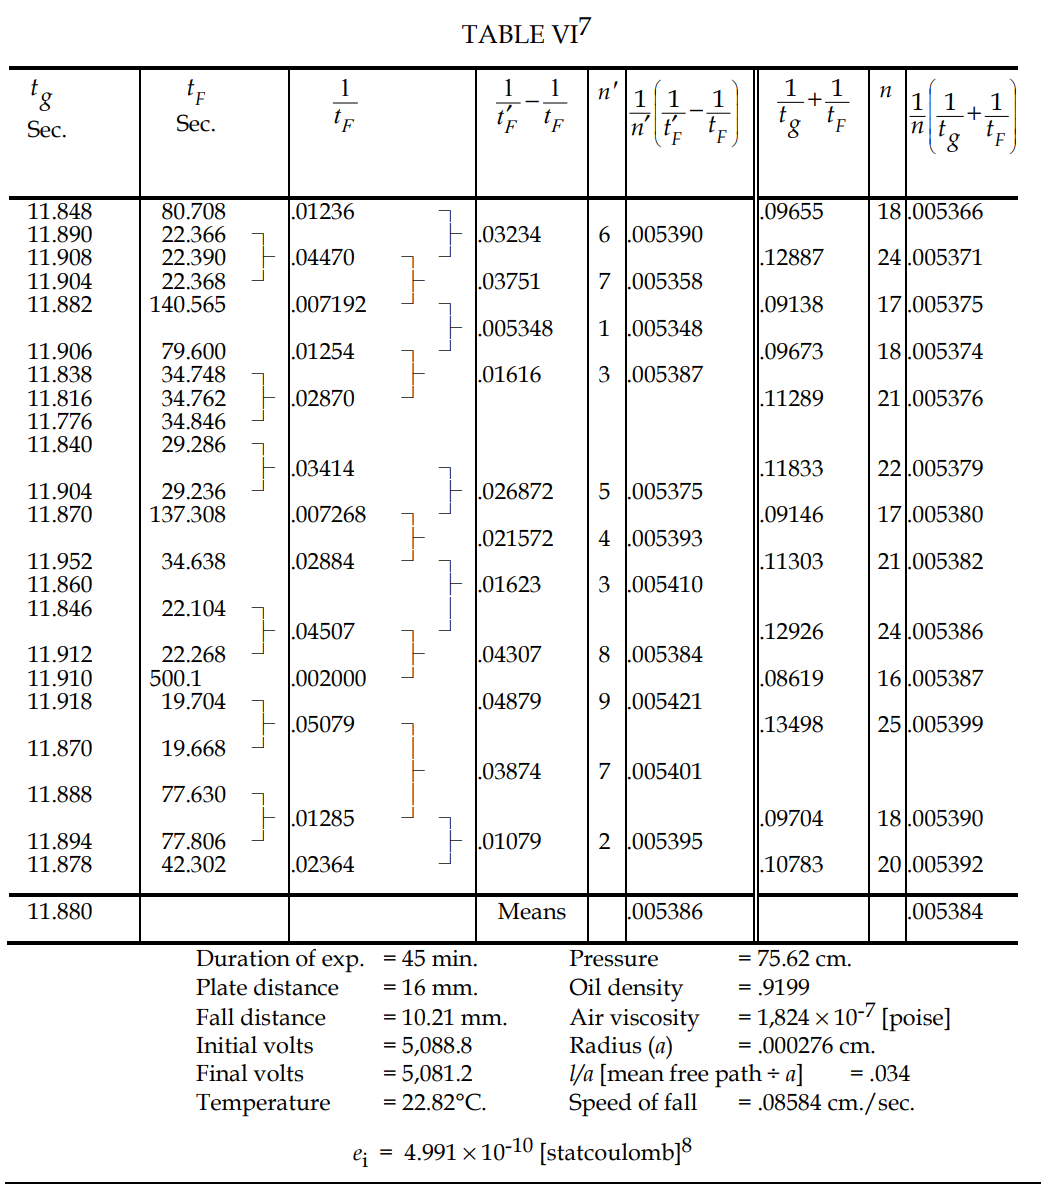
\includegraphics[width=.9\textwidth]{images/03_millikan/table-vi.png}
  \end{center}
\end{figure}
% This is embarrassingly ad hoc: an image of a table I could not figure
% out how to typeset in LaTeX, which included set footnotes. This solution
% is brittle and will not survive if footnotes are added or removed.

\setcounter{footnote}{7}
\footnotetext{[The table entries are given as published; but two
  values are erroneous. In the fourth column, .03874 should be .03794.
  On the same line in the sixth column, .005401 should be .005420. These
  errors do not significantly affect the results.]}

\setcounter{footnote}{8}
\footnotetext{[The value
  presently accepted is $4.802\!\times\!10^-{10}$ statcoulomb.]}

For reasons which will be explained in the next section, each one of
these changes may correspond to the capture of not merely one but of
several distinct ions. The numbers in the fifth column represent simply
the small integer by which it is found that the numbers in the fourth
column must be divided in order to obtain the numbers in the sixth
column. These {[}numbers in the sixth column{]} will be seen to be
exactly alike within the limits of error of the experiment. The mean
value at the bottom of the sixth column represents, then, the smallest
charge ever caught from the air, that is, it is the elementary
\emph{ionic} charge. The seventh column gives the successive values of
$v_1 + v_2$ expressed as reciprocal times. These numbers,
then, represent the successive values of the \emph{total} charge carried
by the droplet. The eighth column gives the integers by which the
numbers in the seventh column must be divided to obtain the numbers in
the last column. These {[}numbers in the last column{]} also will be
seen to be invariable. The mean at the bottom of the last column
represents, then, \emph{the electrical unit out of which the frictional
charge on the droplet was built up, and it is seen to be identical with
the ionic charge represented by the number at the bottom of the sixth
column.}

It may be of interest to introduce one further table (Table VII)
arranged in a slightly different way to show how infallibly the atomic
structure of electricity follows from experiments like those under
consideration.

\begin{center}
\begin{tabular}{c|c|c|c|c|c}
\hline
\multicolumn{6}{c}{TABLE VII}\\
\hline
$n$ & $4.917\!\times\!{n}$ & Observed Charge & $n$ & $4.917\!\times\!{n}$ & Observed Charge\\
\hline
1 & 4.917 & \ldots & 10 & 49.17 & 49.41\\
2 & 9.834 & \ldots & 11 & 54.09 & 53.91\\
3 & 14.75 & \ldots & 12 & 59.00 & 59.12\\
4 & 19.66 & 19.66  & 13 & 63.92 & 63.68\\
5 & 24.59 & 24.60  & 14 & 68.84 & 68.65\\
6 & 29.50 & 29.62  & 15 & 73.75 & \ldots\\
7 & 34.42 & 34.47  & 16 & 78.67 & 78.34\\
8 & 39.34 & 39.38  & 17 & 83.59 & 83.22\\
9 & 44.25 & 44.42  & 18 & 88.51 & \ldots\\
\hline
\end{tabular}
\end{center}

In this table 4.917 is merely a number obtained precisely as above from
the change in speed due to the capture of ions and one which is
proportional in this experiment to the ionic charge. The column headed
4.917 $\times$ \emph{n} contains simply the whole series of exact multiples of
this number from 1 to 18. The column headed ``Observed Charge'' gives
the successive observed values of ($v_1 + v_2$). It will be
seen that during the time of observation, about four hours, this drop
carried all possible multiples of the elementary charge from 4 to 18,
save only 15. \emph{No more exact or more consistent multiple
relationship is found in the data which chemists have amassed on the
combining powers of the elements and on which the atomic theory of
matter rests than is found in the foregoing numbers.}

Such tables as these---and scores of them could be given---place beyond all
question the view that an electrical charge wherever it is found,
whether on an insulator or a conductor, whether in electrolytes or in
metals, has a definite granular structure, that it consists of an exact
number of specks of electricity (electrons) all exactly alike, which in
static phenomena are scattered over the surface of the charged body and
in current phenomena are drifting along the conductor. Instead of giving
up, as Maxwell thought we should some day do, the ``provisional
hypothesis of molecular charges,'' we find ourselves obliged to make all
our interpretations of electrical phenomena, \emph{metallic as well as
electrolytic}, in terms of it.

\subsection*{III. Mechanism of Change of Charge of a Drop}

All of the changes of charge shown in Table IV were spontaneous changes,
and it has been assumed that all of these changes were produced by the
capture of ions from the air. When a negative drop suddenly increases
its speed in the field, that is, takes on a larger charge of its own
kind than it has been carrying, there seems to be no other conceivable
way in which the change can be produced. But when the charge suddenly
\emph{decreases} there is no a priori reason for thinking that the
change may not be due as well to the direct loss of a portion of the
charge as to the neutralization of this same amount of electricity by
the capture of a charge of opposite sign. That, however, the changes do
actually occur, when no X-rays or radioactive rays are passing between
the plates,\footnote{{[}As he elsewhere explains, Millikan repeatedly
  directed x-rays through the chamber or brought radioactive material
  into proximity with it. These measures would greatly accelerate the
  formation of ions in the air and so increase the chances of capturing
  one. But since they might also, by the same token, directly affect the
  charge carried by a droplet, Millikan considers only those changes
  that occur in the absence of such external influences.{]}} only by the
capture of ions from the air, was rendered probable by the fact that
drops not too heavily charged showed the same tendency on the whole to
increase as to decrease in charge. This should not have been the case if
there were two causes tending to decrease the charge, namely, direct
loss and the capture of opposite ions, as against one tending to
increase it, namely, capture of like ions. The matter was very
convincingly settled, however, by making observations when the gas
pressures were as low as 2 or 3 mm. of mercury. Since the number of ions
present in a gas is in general proportional to the pressure,\footnote{{[}That
  the number of \emph{molecules} present in a gas is strictly
  proportional to the pressure, is an element in Avogadro's hypothesis.
  A relatively constant \emph{fraction} of these molecules will become
  ionized under given conditions independent of pressure; hence the
  proportionality cited.{]}} spontaneous changes in charge should almost
never occur at these low pressures; in fact, it was found that drops
could be held for hours at a time without changing. The frequency with
which the changes occur decreases regularly with the pressure, as it
should if the changes are due to the capture of ions. For the number of
ions formed by a given ionizing agent must vary directly as the
pressure.

Again, the changes do not, in general, occur when the electrical field
is on, for then the ions are driven instantly to the plates as soon as
formed, at a speed of, say, 10,000 cm per second, and so do not have
any opportunity to accumulate in the space between them. When the field
is off, however, they do so accumulate until, in ordinary air, they
reach the number of, say, 20,000 per cubic centimeter. These ions, being
endowed with the kinetic energy of agitation characteristic of the
temperature, wander rapidly through the gas and become a part of the
drop as soon as they impinge upon it. It was thus that all the changes
recorded in Table IV took place.\\
\centerline{* * *}
%
\section*{Comment \\
  {\large``Weighing'' the Oil Drop}}

As Millikan shows in his Table V, the two equations
%
\begin{center}
\begin{align*}\tag{9}
\frac{v_1}{v_2} = \frac{mg}{Fe_n-mg} & \: & \text{or} & \: & e_n = \frac{mg}{Fv_1}(v_1+v_2)
\end{align*}
\end{center}
%
and
%
\begin{equation}\tag{10}
e_i = e_{n'}-e_n=\frac{mg}{Fv_1}(v_{2}'-v_2)
\end{equation}
%
suffice to determine \emph{relative} values for $e_n$ (total charge
on an oil drop) and $e_i$ (charge of a captured ion), using nothing
more than stopwatch measurements on the motion of the drop. The
equations will determine \emph{exact} values for those charges as well;
but only if he can evaluate \emph{mg}, the ``effective'' weight of the
drop in a buoyant medium, which we have already expressed above as
%
\begin{equation*}
mg = V(\sigma\!-\!\rho)g
\end{equation*}
%
or, assuming the drop to be a sphere of radius \emph{a},
%
\begin{equation*}\tag{3.6}
mg = \frac{4\pi{a}^3}{3}(\sigma\!-\!\rho)g.
\end{equation*}
%
Millikan has no way to measure this quantity directly; but reasoning
from the viscous (resistive) properties of the medium, air, he is able
to devise an indirect measurement.

We have already derived in equation (3.3) an expression for the limiting 
velocity attained by a body that falls through a viscous medium:
%
\begin{equation*}\tag{3.3}
v_1 = \frac{mg}{R}
\end{equation*}
%
where $R$ is a so far unspecified proportionality constant. This
constant is different for every different-sized oil drop. However,
Millikan was able to relate it to a general, measurable quantity. The
\emph{viscosity} of a fluid is its resistance to being passed through,
as we mentioned, or to flowing past something. This property can be more
precisely defined and measured by various procedures.\footnote{The
  details are beyond our scope.} Accurate tables of the viscosity of air
were available to Millikan. In addition, \emph{Stokes's Law} (derived by
George Stokes in 1845) applies this property to the case of a smooth
sphere moving through a fluid. Millikan assumed that his oil drops were
spheres; with air viscosity $\eta$ and drop radius $a$, Stokes's
Law gives $R = 6\pi \eta a$.\footnote{Again, we cannot follow the
  details.} Substituting into Eq. 3.3) gave Millikan
%
\begin{equation*}\tag{3.7}
v_1 = \frac{mg}{6\pi\eta a}.
\end{equation*}
%
He then eliminated \emph{a} between equations (3.6) and (3.7) to obtain
%
\begin{equation*}
m = \frac{4\pi}{3}(\sigma\!-\!\rho)\left(\frac{mg}{6\pi\eta v_1}\right)^3,
\end{equation*}
%
from which
%
\begin{equation*}
\left(\frac{mg}{v_1}\right)^2 = \frac{3\cdot6^3\pi^2\eta^3{v}_1}{4g(\sigma\!-\!\rho)}.
\end{equation*}
%
Hence for the coefficient $mg/Fv_1$ in Millikan's equations (9) and (10) we have
%
\begin{equation*}\tag{3.8}
\frac{mg}{Fv_1} = \left(\frac{9\pi}{F}\sqrt{\frac{2\eta^3}{g(\sigma\!-\!\rho)}}\right)\cdot\sqrt{v_1}
\end{equation*}
%
which is sufficient to evaluate $e_n$ and $e_i$.

\section*{Experiment: Measurement of the ``Atom of Charge''}

We use the Pasco oil-drop apparatus, which is similar to Millikan's,
only far smaller. In addition, the viewing telescope and associated
illumination are integrally mounted. Make sure that the apparatus is
level, the telescope illumination \emph{on}, and the high voltage
\emph{off}. If the following preliminary adjustments have not already
been made by the laboratory assistant, perform them now:

\emph{Focus the telescope:} Remove the chamber housing, lid, and droplet
hole mask, as illustrated in the drawing. Unscrew the focusing wire from
its storage position and carefully insert it into the droplet hole in
the center of the upper plate. Adjust the Reticle Focusing Ring on the
telescope to bring the viewing reticle into focus. Adjust the Droplet
Focusing Ring to bring the wire image into sharp focus. When the
telescope is focused, each minor reticle division corresponds to a
droplet fall distance of .01 cm; each major division to .05 cm.

\emph{Focus the lamp:} Turn the lamp's Horizontal Adjustment to bring
the right edge of the wire into highest contrast compared to the center
of the wire. Turn the Vertical Adjustment to direct the brightest light
onto the part of the wire that is within the reticle. Remove and return
the focusing wire to its storage position and reassemble the chamber.

\begin{wrapfigure}[18]{r}{2.45in} % this can appear anywhere in this subsection
										  % move if necessary
  \begin{center}
    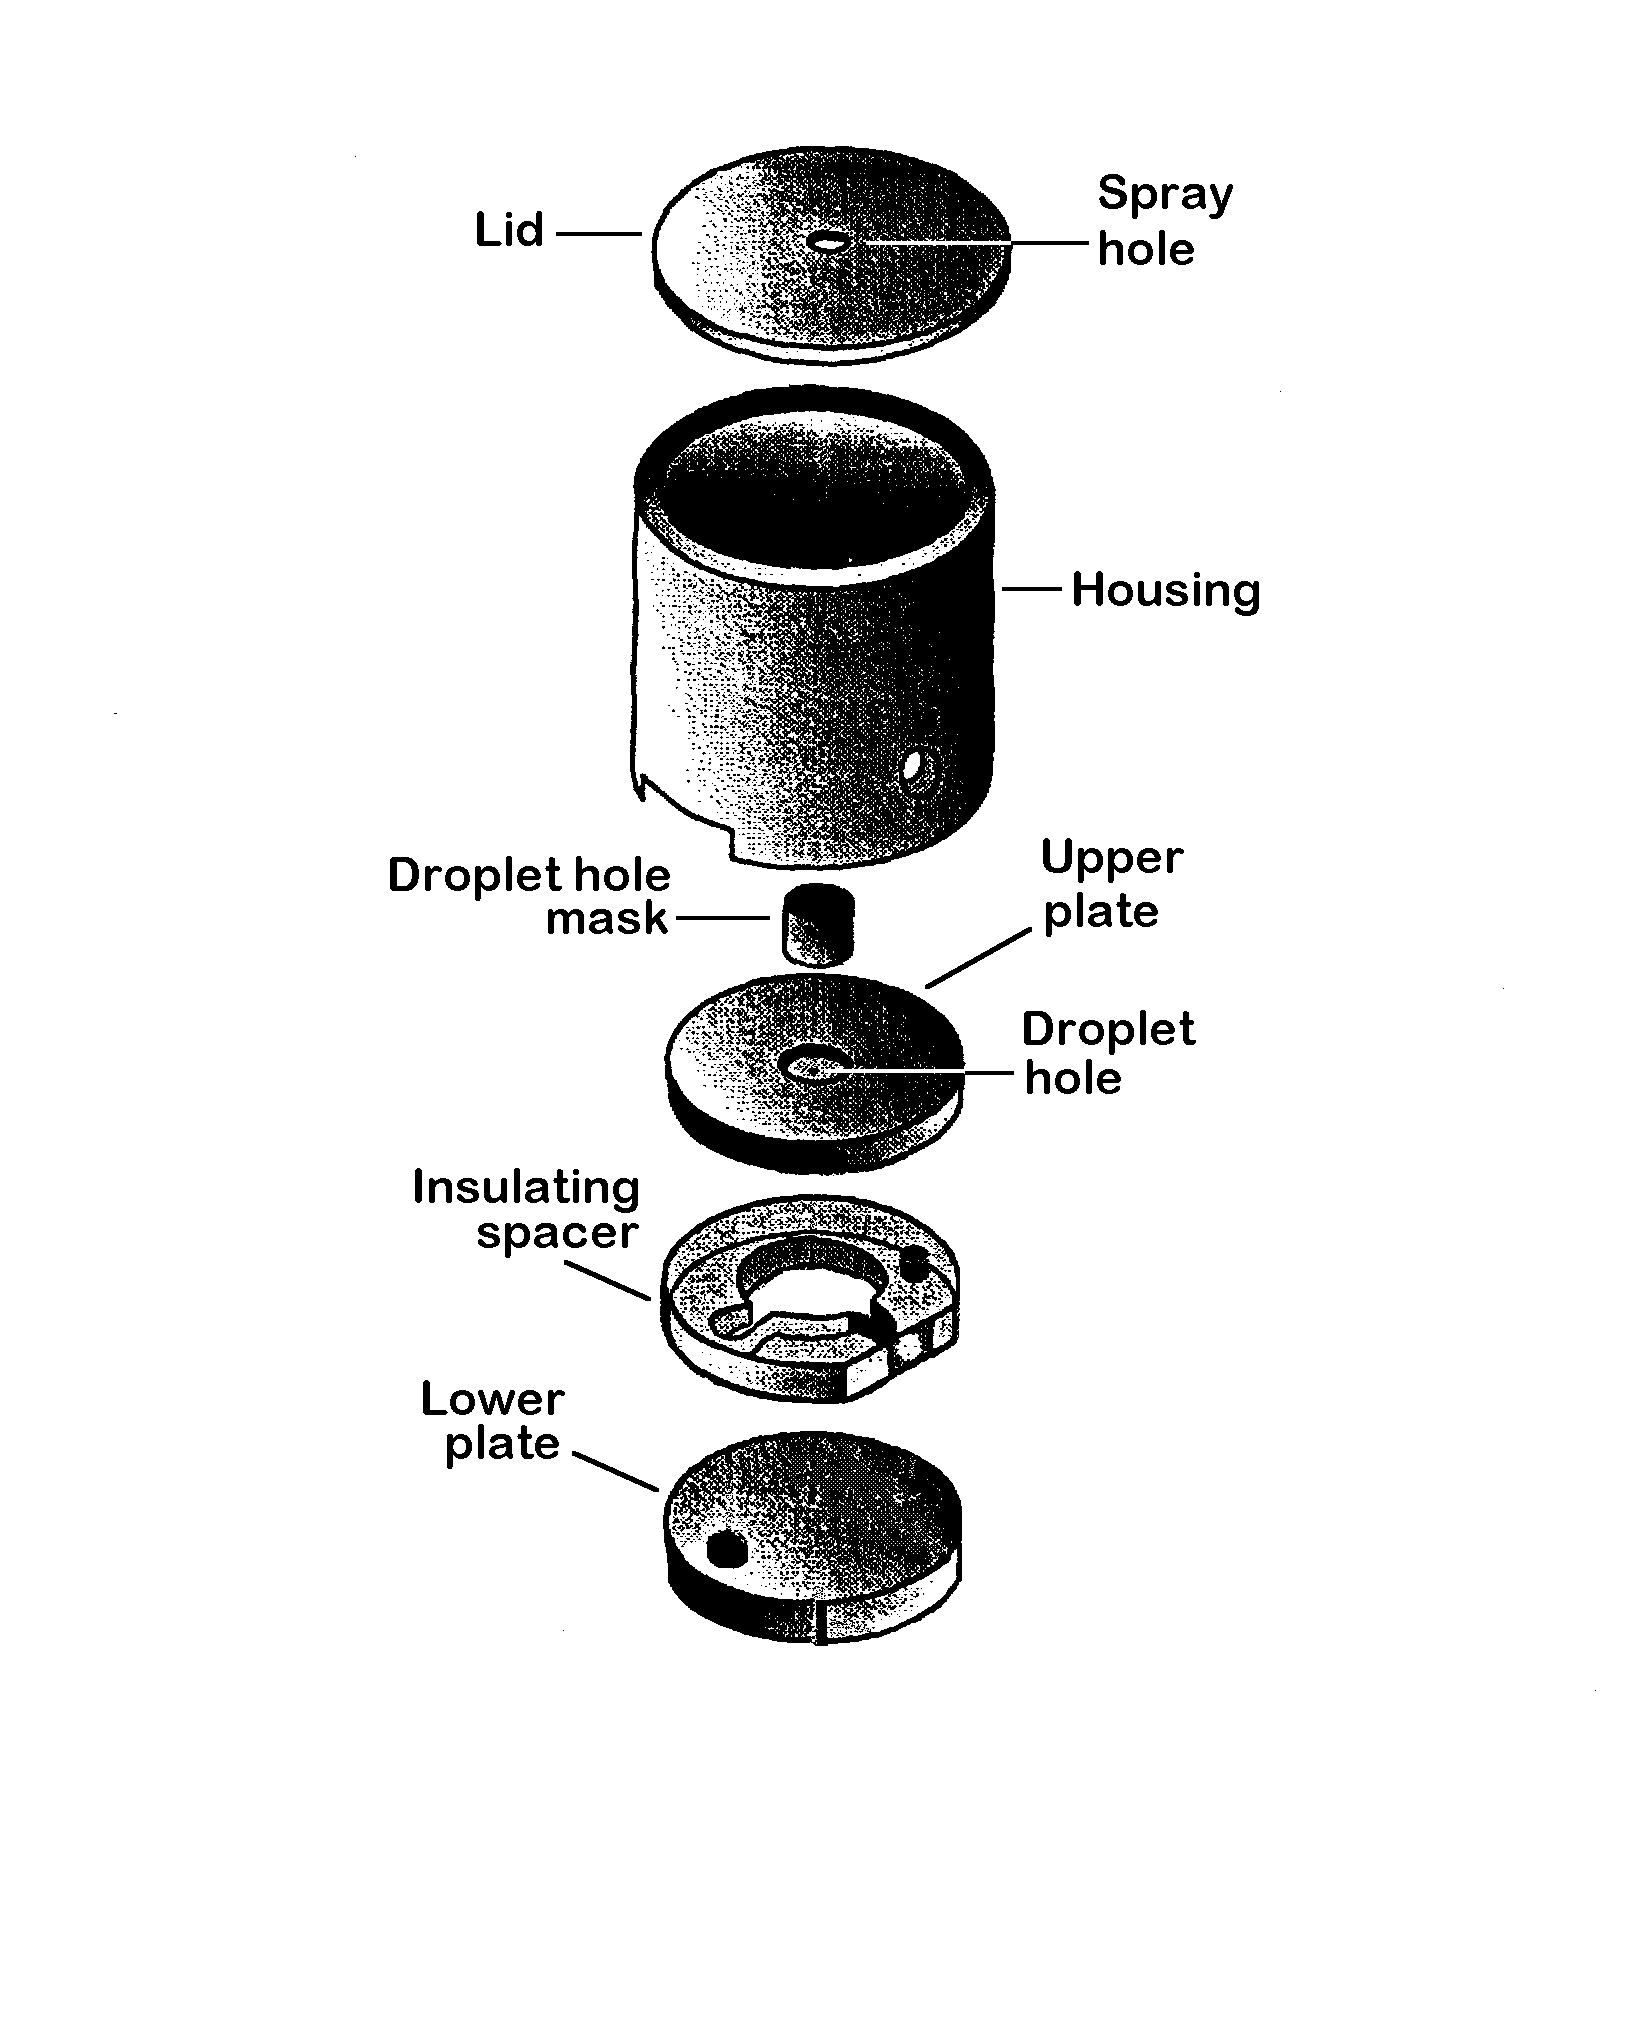
\includegraphics[width=2.33056in,height=3.38264in]{images/03_millikan/image067.png}
  \end{center}
\end{wrapfigure}

\emph{Adjust the plate voltage:} Connect the high-voltage supply. Turn
the cable-mounted plate switch to the GROUNDED position. Adjust the
supply to deliver between 400 and 500 volts, and record the voltage. The
apparatus is now ready for use.

Begin by introducing oil droplets into the chamber. Move the vent lever
to the Spray Droplets position; this will permit air to escape from the
chamber as the oil spray enters. The atomizer nozzle should be turned
vertically downward. After one or two test squeezes to make sure oil
sprays correctly, point the nozzle into the spray hole in the lid of the
chamber.

While looking through the telescope, give the atomizer \emph{one quick
squeeze}, followed im\-me\-di\-ate\-ly by \emph{one slow squeeze} to create a
vertical downdraft. When you see a shower of drops through the
telescope, move the vent lever to the OFF po\-si\-tion.\footnote{Avoid
  immoderate use of the atomizer. The object is to introduce a small
  number of drops, from which a single drop can be chosen. If a large,
  bright cloud appears in the viewing area, spraying has been excessive.
  You can try waiting a few minutes to see if the drops settle out of
  view, but most likely the chamber will have to be disassembled and
  cleaned.}

With a number of drops in view, observe that different drops fall with
noticeably different speeds. This illustrates the relation expressed in
equation (3.3)---heavier drops fall proportionately faster than lighter
ones. Pay attention to those droplets that fall \emph{slowly}---about
10--25 seconds to travel the distance between major reticle lines (.05
cm).

Energizing the plates will reveal which drops bear a charge, and whether
the applied voltage is in the right direction to \emph{reverse} a drop's
falling motion (which is desired) or not. Repeatedly move the
cable-mounted plate switch to its + or -- positions. When a droplet is
found that can be driven back towards the upper plate by applying the
voltage, try to keep it in capture by alternately applying and removing
that voltage.

\subsubsection*{Measurements on a single drop}

Execution of the experiment will require two people, one to observe the
drop and operate the stopwatch, the other to read the watch and record
the timed intervals. It is usually best to time successive rising and
falling transits of the droplet over any \emph{major} (.05 cm) division
on the telescope's viewing reticle---ten to twenty measurements in each
direction are desirable. Do not raise or lower the plate voltage
adjustment once you begin timing a drop. Record the fall times and rise
times in separate columns. A series of measurements of these times,
\emph{all performed on the same drop}, will enable you to construct a
table like Millikan's Table VI. Here is an example (figures are from
1997):

\begin{center}
\small
\begin{tabular}{|l|c||c|c|c|c|c|c|c|c|}
\hline
 & $d$ = 0.5cm & & $d$ = 0.5cm & \makecell{Charge\\on ion} & & & \makecell{Frictional\\charge} & & \\
\hline
$t_g$ & \makecell{$v_1(=d/t_g)$\\(cm/sec)} & $t_F$ & \makecell{$v_2(=d/t_F)$\\(cm/sec)} & $(v_{2}'\!-\!v_2)$ & $n'$ & $\frac{v_{2}'-v_2}{n'}$ & $v_1+v_2$ & $n$ & $\frac{v_1+v_2}{n}$\\
\hline
18.2    & .00286 & 3.8 & 0.01316 & & & & 0.01602 & 3 & .00534\\
18.6    & \emph{avr}  & & & .00470 & 1 & .00470 & & & \\
19.2    & & 2.8 & .01786 & & & & & & \\
18.0    & & & & .01561 & 3 & .00520 & & & \\
17.2    & & 22.2 & .00225 & & & & & & \\
15.4    & & & & .00544 & 1 & .00544 & & & \\
16.7    & & 6.5 & .00769 & & & & & & \\
18.0    & & & & .00541 & 1 & .00541 & & & \\
15.4    & & 21.9 & .00228 & & & & & & \\
17.3    & & & & .01123 & 2 & .00562 & & & \\
\underline{18.4}    & & 3.7 & .01351 & & & \underline{\hspace{2em}} & & & \underline{\hspace{2em}} \\
17.5 & & & & & & .00527 & & & .00534 \\
\emph{avr} & & & & & & \emph{avr} & & &\\
\hline
\end{tabular}
\end{center}

\subsubsection*{Measurements on Multiple Drops}

Although it would be convenient to make all measurements on a single
droplet, it is seldom possible to do so; for it proves extremely
difficult to hold any one drop in play for long periods of time. But
droplets of the same material differ from one another only in mass.
Therefore---see Equation 3.8 above---if the electric field intensity
\emph{F} is not changed, the coefficient in Millikan's equations (9) and
(10) will vary, from drop to drop, only in proportion to $\sqrt{v_1}$. You may
therefore combine data from different drops by tabulating and comparing
\begin{center}
\begin{tabular}{ c c c }
$\sqrt{v_1}(v_1+v_2)$ & and & $\sqrt{v_1}(v_{2}'-v_2)$\\
\end{tabular}
\end{center}
instead of (\emph{v}\textsubscript{1} + \emph{v}\textsubscript{2}) and
(\emph{v}'\textsubscript{2} -- \emph{v}\textsubscript{2}) directly. Here
is an example of such a table (the figures are from 1983):

\begin{center}
\small
\begin{tabular}{l l l l l l}
\hline
Obsvd. $t_g$ & $v_1$ (i.e., $1/t_g$) & Obsvd. $t_F$ & $v_2$ (i.e., $1/t_F$) & $(v'_2-v_2)$ & $\sqrt{v_1}(v'_2-v_2)$\\
\hline
7.2 sec & .1389 & 2.1 sec & .4762 & .1984 & .0739\\
 & & 3.6 & .2778 & .1978 & .0737\\
 & & 12.5 & 0.0800 & &\\
5.8 sec & .1724 & 1.9 & .5263 & .3792 & .1575\\
 & & 6.8 & .1471 & .8529 & .3541\\
 & & 1.0 & 1.000 & .7059 & .2931\\
 & & 3.4 & .2941 & &\\
\end{tabular}
\end{center}

The table entries reflect measurements on two different droplets. In the
sixth column the observed changes in rise speed are multiplied by
$\sqrt{v_1}$ as explained above. The resulting quantities
are very nearly integral multiples of about .076. This trial, therefore,
would indicate the existence of a fundamental ionic charge, with a
relative value of about .076.

\subsubsection*{Enhancing Ionization}

It is hoped that the droplet will acquire an ion during one of its
falls, as is indeed illustrated in the foregoing
chart. Capture of an ion does not change the drop's falling velocity,
but it will change the drop's rising velocity when the plate voltage is
next applied. However, should you find that your droplet has not caught
an ion after 10--20 successive rises, move the vent lever to the
IONIZATION ON position for a few seconds during the next fall period.
That will expose the air in the chamber to a low-level radioactive
thorium source, thus increasing the number of ionized particles in the
air and multiplying the chances for the falling drop to encounter an
ion. Repeat the exposure if again the drop fails to capture an ion after
10-20 measurements, and continue for as long as the droplet can be held
in play. It is desirable to measure as many different charges on a
single drop as possible.

\subsubsection*{Frictional Charge and Ionic Charge}

As Millikan explains, the \emph{initial} charge on a droplet, prior to
the capture of an ion, must have been acquired by friction during the
spraying process. In the foregoing chart it is assumed that the first
measurement made on the drop reflects this initial frictional charge.
While that may be a reasonable assumption provided the first measurement
was made \emph{soon} after spraying, and the observed frequency of ion
capture by a drop is not high, remember that it is \emph{only} an
assumption---the drop may have already picked up an ion by the time we
first measure it. That is especially to be suspected when, as in this
example, the apparent number $n$ of unit charges on the drop is
only \emph{3}---a number so small it could as easily reflect ion capture
as frictional electrification.

If it is desired to measure \emph{frictional charges specifically}, do
not use the ionization source---we want to minimize the chances of
capturing an ion. As soon after spraying as possible, try to select a
drop whose rising velocity is noticeably \emph{faster} than others.
Rapid rising indicates a high charge, which is more likely to have been
frictionally acquired. As before, time the drop for 10--20 transits, or
until it appears to have en\-coun\-tered an ion. Let the drop escape; spray
again, and repeat the measurements on another drop.

\subsubsection*{Calculation of the Fundamental Charge}

The stopwatch measurements illustrated in the previous chart suffice to
determine values of and which, as Millikan's equations (9) and (10) make
clear, are proportional to the \emph{initial frictional charge on a
drop} and the \emph{charge on a captured ion}, respectively. But in
order to calculate exact values of these charges, not just relative
ones, we must evaluate the coefficient that appears in those equations.
By our equation 3.8 above, the coefficient can be calculated
from the following quantities:

\begin{quote}
(a) the velocity $v_1$ of the falling drop. This you have already
measured; just remember to cite the correct value for each different
drop. (Remember to average and to take the square root.)

(b) the electric field intensity $F$ between the plates. To compare our 
results numerically with Millikan's we will calculate this in e.s.u., 
so we must express the potential difference between the
plates in e.s.u., i.e.\ in \emph{statvolts}. Our meters give volts and 1
volt = 1/300 statvolts, so \emph{the voltmeter reading must be divided
by 300}. The plate separation is 0.76 cm, unless a different value is
labeled on the side of your apparatus. Then the voltage in statvolts
divided by the plate separation in cm will give electric field intensity
in e.s.u.\footnote{See Appendix for an explanation of the units and for the
  relation between $F$ and the potential difference.}

(c) the density of the oil, $\sigma$. We use Squibb \#5597 non-volatile
mineral oil, for which $\sigma = .886\ \text{g/cm}^3$.

(d) the density of the air, $\rho$, obtained from the graph below. You
will have to note the temperature of the air in the chamber and the 
barometric pressure in the room. Typical values for
$\rho$ are about $.0012\ \text{g/cm}^3$.

(e) the viscosity of the air, $\eta$, obtained from the graph below.
Typical values for $\eta$ are around $1825\ \times\ 10^{-7}\ \text{poise (gm/cm-sec)}.$

(f) the acceleration of gravity, $g = 980\ \text{cm/sec}^2$.
\end{quote}


\begin{figure}[h]
  \begin{center}
    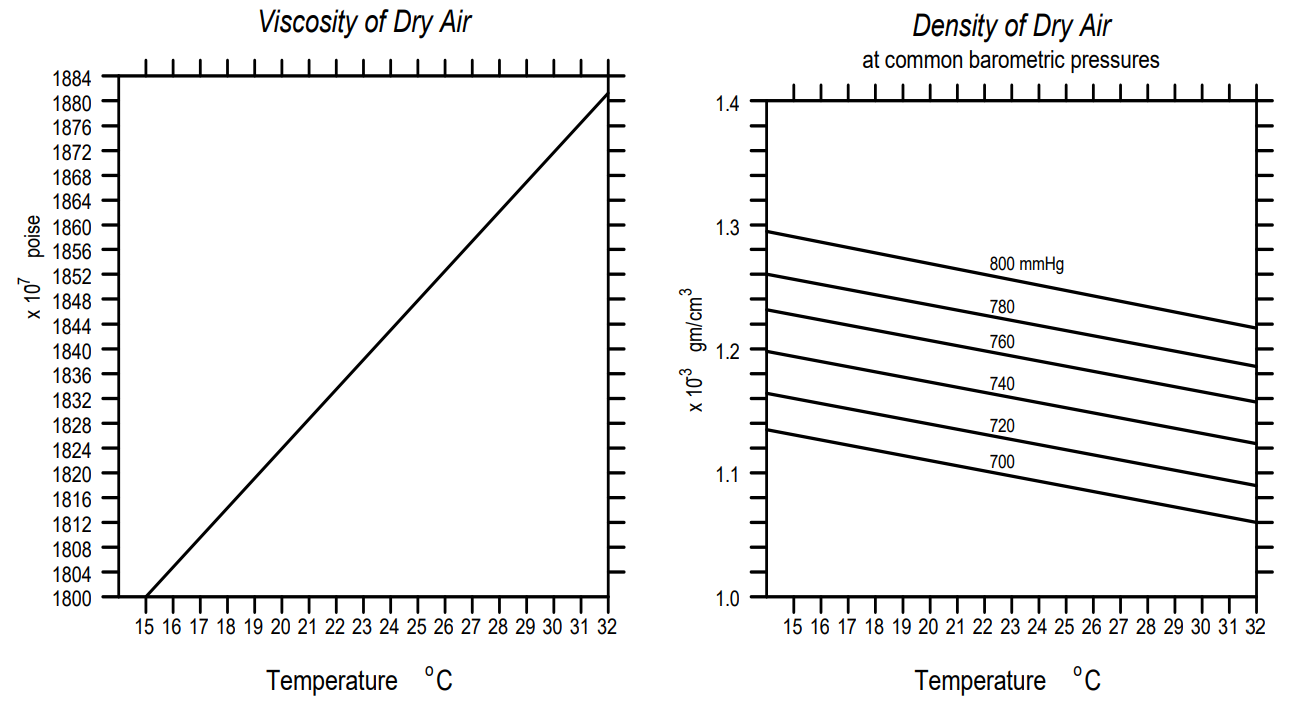
\includegraphics[width=0.9\textwidth]{images/03_millikan/image100.png}
  \end{center}
\end{figure}


%\includegraphics[width=5.53889in,height=3.07847in]{media/image47.wmf}

\subsubsection*{Remarks on Avogadro's Number}

As Millikan himself pointed out, mere \emph{measurement} of the
fundamental charge is not necessarily, in itself, the most important
fruit of this experiment. Of far greater con\-se\-quence, perhaps, is the
demonstration that the same ``electron'' lies at the root of both
\emph{static electricity} (the frictional charge on the drop) and
\emph{chemical activity} (the ionic charge). This is strong, even
conclusive evidence, for the interpretation of chemical power as being
fundamentally electrical, for Millikan's results indicate that the
\emph{fundamental unit of charge} corresponds also to the
\emph{fundamental unit of chemical combining power}. If the electron has
indeed this dual significance, then Millikan's measurement of the
electron charge will at last permit accurate calculation of that
theoretically pivotal but ex\-per\-i\-men\-tal\-ly elusive quantity,
\emph{Avogadro's number}---the number of atoms in a gram-atomic weight
of any element.\footnote{There had been earlier efforts to estimate
  Avogadro's number, predating Millikan's oil-drop measurements;
  Einstein cites one of his own in his paper that appears in Chapter VI
  below. But the most reliable determinations of Avogadro's number and
  many other constants all depend on accurate knowledge of the electron
  charge (cf.\ \emph{The Electron}, Chapter X).}

Recall that the ``equivalent weight'' of an element is that much of it,
measured on the scale of atomic weights with Hydrogen = 1, which
exercises \emph{one unit} of chemical combining power. But the combining
power of one hydrogen atom is taken as the unit for chemical combining
power generally; thus for hydrogen and all atoms equal to hydrogen in
their combining power, the atomic weight and the equivalent weight are
the same.\footnote{Chemical combining power is commonly expressed in
  units of ``valence''; hydrogen and all atoms equivalent to it are said
  to be \emph{univalent} atoms.}

Now if one unit of chemical combining power actually means \emph{one
electron of electric charge}, then one gram-atomic weight of hydrogen
will exercise the cumulative charge of Avogadro's number of electrons,
which is
%
\begin{equation*}
N_0\!\times\!e,
\end{equation*}
%
where $N_0$ denotes Avogadro's number and \emph{e} is the electron
charge. Now the above is also the total charge associated with a
gram-equivalent weight of hydrogen, since for it the gram-atomic weight
is equal to the gram-equivalent weight. But we found in electrolysis
that the total charge associated with liberation or transfer of one
gram-equivalent weight of \emph{any} element is 96,500 coulombs, which
equals $2.895 \times 10^{14}$ stat\-cou\-lombs; hence we may write
%
\begin{equation*}
2.895 \times 10^{14} \text{ statC} = N_0\!\times\!e
\end{equation*}
%
While Millikan has shown that (modern value):
\begin{equation*}
e = 4.802\!\times\!10^{-10} \text{ statC}
\end{equation*}
Thus we have
\begin{equation*}
N_0 = \text{Avogrado's number} = \frac{2.895\!\times\!10^{14}}{4.802\!\times\!10^{-10}} = 6.028\!\times\!10^{23}.
\end{equation*}
(Other, more recent, determinations yield $6.023\!\times\!10^{23}$.)

\subsubsection*{Weighing and Sizing Elementary Particles}

Determination of Avogadro's number puts us in a position to ``weigh all
the atoms''; for if there are $N_0$ atoms in a gram-atomic weight of
an element, then each atom must weigh $1/N_0$ of the gram-atomic
weight. For example, a gram-atomic weight of hydrogen weighs 1.008
grams. Then a single hydrogen atom, for example, must weigh
\begin{equation*}
1.008 \div (6.023\!\times\!10^{23}) = 1.674\!\times\!10^{-24} \text{ g}
\end{equation*}
and similarly for all the other atoms.

In Chapter II of \emph{The Electron} Millikan pointed out that the term
``electron'' had been first introduced in 1891 as a name for the
supposed ``natural unit of electricity,'' namely, that quantity of
electricity exhibited by a hydrogen ion or any other univalent ion. Thus
it denoted simply a \emph{definite quantity of electricity} without
reference to any mass or inertia which might be associated with it. It
is clear that Millikan's oil-drop experiment has proved the existence of
``electron'' in this original sense.

But measurements by Thomson and others of the charge-to-mass ratio of
ions in both gases and liquids strongly implicated Thomson's
\emph{cathode-ray corpuscle} as the es\-sen\-tial constituent whereby atoms
acquire either an excess or deficiency of negative charge to become
ions.\footnote{See note 5 above; Millikan devotes the whole of
  his Chapter II to this very interesting story.} This implies that
\emph{the charge borne by each cathode ray corpuscle must be the very
quantity of charge that had been termed ``electron.''} As a result,
Millikan explains, the word ``electron'' gradually changed its meaning
to become synonymous with the cathode-ray corpuscle: a particle having
definite mass as well as charge, a constituent not only of cathode rays
but of atoms themselves.\footnote{Millikan views this alteration of
  usage with real distress: ``It is unfortunate that modern writers have
  not been more careful to retain the original significance of
  {[}`electron'{]}, for it is obvious that a word is needed which
  denotes merely the elementary unit of electricity and has no
  implication as to where that unit is found, to what it is attached,
  with what inertia it is associated, or whether it is positive or
  negative in sign.''} Since the electron (in the new sense of
\emph{particle}) has the charge-to-mass ratio that was determined for
cathode-rays, and has, on the other hand, the quantity of charge that is
disclosed in Millikan's experiment, we are able to calculate its mass,
to ``weigh'' the electron itself.

We have, from the cathode rays,
\begin{equation*}
m/e = .5685 \times 10^{-7} \text{g/abC} = 1.895 \times 10^{-18} \text{ g/statC}.
\end{equation*}
Then, since the electron charge is
\begin{equation*}
e = 4.802 \times 10^{-10} \text{ statC},
\end{equation*}
we may calculate
\begin{equation*}
m = 1.895 \times 10^{-18} \times 4.802 \times 10^{-10} = .9099 \times 10^{-27} \text{ g}.
\end{equation*}
Hence the electron will be almost 1840 times lighter than the hydrogen
atom. That an electron weighs such a slight fraction of even the
lightest atom will prove important in formulating a conception of the
atom's structure, as discussed in Rutherford's paper which follows.

\subsubsection*{``Sizing'' an Atom}

Another magnitude interesting in itself and also important in
Rutherford's paper is the approximate \emph{size} of an atom. Using
Avogadro's Number this is easy to calculate for elemental solids.

Take gold, which is what Rutherford will be dealing with. The density of
gold is 19.3 g/cm\textsuperscript{3}, while its gram-atomic weight is
197. Therefore there are .098 gram equivalents in a cubic centimeter of
gold. But since there are $N_0$ atoms in a gram-atomic weight of an
element, we can now say that there are $.098 \times (6.023 \times 10^{23})$, or $5.90 \times
10^{22}$, atoms in a cubic centimeter of gold. Each atom
thus occupies a volume of $1/(5.90 \times 10^{22}) = 1.69 \times
10^{-23}$ cubic centimeters. The cube root of this, $2.57 \times
10^{-8}$ cm, will give the side of a cube of this volume.
Let us assume that gold atoms are spherical and that in solid gold they
fit together in a more or less cubical pattern. Then half of $2.57 \times
10^{-8}$ cm, i.e.\ 
\begin{equation*}
1.285 \times 10^{-8} \text{ cm},
\end{equation*}
is a reasonable rough estimate for the radius of a gold atom. Rutherford
implicitly adopts this size estimate as he analyses how particles that
are \emph{much smaller} than this interact with gold atoms.
